In order to increase the speed of our program, we have decided to parallelize it on a set of cluster of multicore machines. But there is many ways of parallelize our algorithm and we have to choose how we want to do it. 
\subsubsection{Previous Work}
In the last report, we talked about the different methods, their advantages and drawbacks. We have seen that there is mainly two parallelization methods that are efficient.
\newline
\newline
The first one is called the Root Parallelization. It consists in giving the tree to develop to every threads, let them develop it randomly without any communication with the environment
during a certain amount of time and then, merge the results of each tree.
This method has the great benefit of reducing at maximum the communication between the actors, in this case, the threads.
There's only a communication at the beginning and at the end, without needing any synchronization. The Root Parallelization is depicted in figure \ref{root}.\newline

%\begin{figure}[!h] 
%\centerline{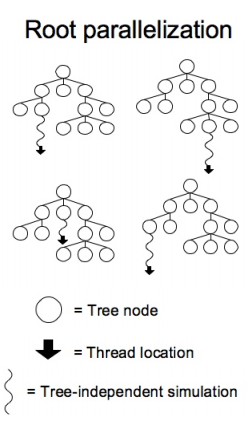
\includegraphics[scale=0.60]{root.png}}
%   \caption{\label{étiquette} Overview of Root Parallelization}
%\label{root}
%\end{figure}

The other efficient parallelization method is called UCT-Treesplit and is depicted if figure \ref{treesplit}. It looks like Root Parallelization as we give to each actor the same tree to develop.
Contrary to Root Parallelization, when the tree is develop on certain node, it goes on working packages who are distributed among every actor.
In terms of performance, this method is very efficient but need an High-Performance Computer, or HPC, and is very sensitive to network latency. \newline

%\begin{figure}[!h] 
%\centerline{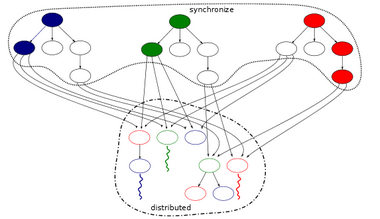
\includegraphics[scale=0.60]{treesplit.png}}
%   \caption{\label{étiquette} Overview of UCT-Treesplit Algorithm}
%\label{treesplit}
%\end{figure}


We have to choose two parallelization methods, one for the cluster parallelization and another for the shared memory parallelization.
\subsubsection{Cluster Parallelization}
For the cluster parallelization, we have to take into account the fact that we will need to communicate by sending messages, so it is relatively costly.
Moreover, as the network can have latency we should minimize the communication between the computers and that's why we have choose to implement a Root Parallelization.
It reduces the cost in communication at maximum, is very simple to implement,it does not depend of configuration of each computer and is very efficient.
\subsubsection{Shared Memory Parallelization}
For the shared memory parallelization we could choose both Root Parallelization or UCT-Treesplit.
If we choose UCT-Treesplit, we may not success to implement it correctly since it is a very complex strategy and, moreover, we would be very sensitive to the problems of the network. In this case, we will implement another Root Parallelization : it will be BLA BLA.
